\subsection*{Task 1}

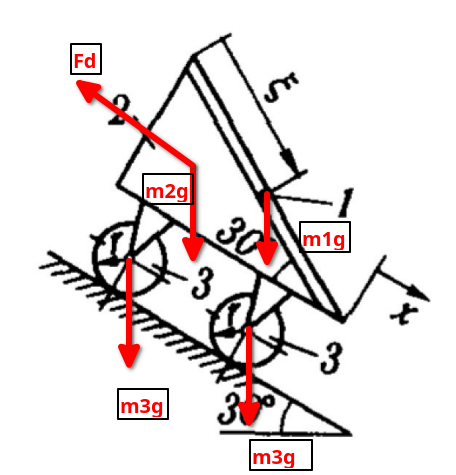
\includegraphics[width=0.5\linewidth]{task1.png}

\begin{enumerate}
    \item RO: System of 4 bodies: particle 1 (translatory),
          body 2 (trnaslatory), wheel $3_1$, wheel $3_2$ (planar)
    \item Method: analytic mechanics - Euler-Lagrange $2_{nd}$ order
    \item Kinematics analysis: 2 dof - $q_1 = x$, $q_2 = \xi$
    \item Force analysis: active forces are only:
          $\vec{P}_1$, $\vec{P}_2$, $\vec{P}_{3_1}$, $\vec{P}_{3_2}$, $\vec{F}_d = -b \vec{v}$
    \item Solution:
          \begin{enumerate}
              \item Euler-Lagrange equations:
                    \begin{align}
                        \begin{cases}
                            \frac{d}{dt} \frac{\partial T}{\partial \dot{q}_1} - \frac{\partial T}{\partial q_1} = -\frac{\partial \Pi}{\partial q_1} + Q_{q_1}
                            \\[10pt]
                            \frac{d}{dt} \frac{\partial T}{\partial \dot{q}_2} - \frac{\partial T}{\partial q_2} = -\frac{\partial \Pi}{\partial q_2} + Q_{q_2}
                        \end{cases}
                    \end{align}
              \item Kinetic energy energy:
                    \begin{align}
                        J_3 = \frac{1}{2} m_3 r^2                                                                     \\
                        T = \frac{m_1}{2} (\dot{x}^2 + \dot{\xi}^2 + 2\dot{x}\dot{\xi} \cos(\alpha)) + \
                        \frac{m_2}{2} \dot{x}^2 + 2 (\frac{m_3}{2} \dot{x}^2 + \frac{1}{2} J_3 (\frac{\dot{x}}{r})^2) \\
                        T = \frac{m_1}{2} (\dot{x}^2 + \dot{\xi}^2 + 2\dot{x}\dot{\xi} \cos(\alpha)) + \
                        \frac{m_2}{2} \dot{x}^2 +  \frac{3 m_3}{2} \dot{x}^2
                    \end{align}
              \item Potential energy:
                    \begin{align}
                        \Pi = -P_1 (x \sin(\alpha) + \xi \cos(\alpha)) - P_2 x \sin(\alpha) - 2 P_{3} x \sin(\alpha)
                    \end{align}
              \item Generalized forces: \\
                    I compute generalized forces through work:
                    \begin{align}
                        \begin{cases}
                            \delta A_{q_1} = Q_{q_1} \cdot \delta q_1 \\
                            \delta A_{q_2} = Q_{q_2} \cdot \delta q_2
                        \end{cases}
                    \end{align}
                    The only non potential forces on generalized coordinates would be:
                    \begin{align}
                        \begin{cases}
                            Q_{q_1} = -b \dot{x} \\
                            Q_{q_2} = 0
                        \end{cases}
                    \end{align}
              \item Compute everything:
                    \begin{align}
                        \frac{\partial T}{\partial \dot{q_1}} = (m_1 + m_2 + 3 m_3) \dot{x} + \dot{\xi} m_1 \cos(\alpha)                \\
                        \frac{\partial T}{\partial \dot{q_2}} = m_1 \dot{\xi} + m_1 \dot{x} \cos(\alpha)                                \\
                        \frac{d}{dt} \frac{\partial T}{\partial \dot{q_1}} = (m_1 + m_2 + 3 m_3) \ddot{x} + \ddot{\xi} m_1 \cos(\alpha) \\
                        \frac{d}{dt} \frac{\partial T}{\partial \dot{q_2}} = m_1 \ddot{\xi} + m_1 \ddot{x} \cos(\alpha)                 \\
                        \frac{\partial T}{\partial q_1} = 0                                                                             \\
                        \frac{\partial T}{\partial q_2} = 0                                                                             \\
                        \frac{\partial \Pi}{\partial q_1} = (P_1 + P_2 + 2 P_3) \sin(\alpha)                                            \\
                        \frac{\partial \Pi}{\partial q_2} = P_1 \cos(\alpha)
                    \end{align}
              \item Substitute into (1) and chill:
                    \begin{align}
                        \begin{cases}
                            (m_1 + m_2 + 3 m_3) \ddot{x} + \ddot{\xi} m_1 \cos(\alpha) = (P_1 + P_2 + 2 P_3) \sin(\alpha) - b \dot{x} \\
                            m_1 \ddot{\xi} + m_1 \ddot{x} \cos(\alpha) = P_1 \cos(\alpha)
                        \end{cases}
                    \end{align}
                    This is already enough to complete this task, only thing left is to solve this system of equations.
              \item Plot of $x(t)$ and $\xi(t)$: \\
                    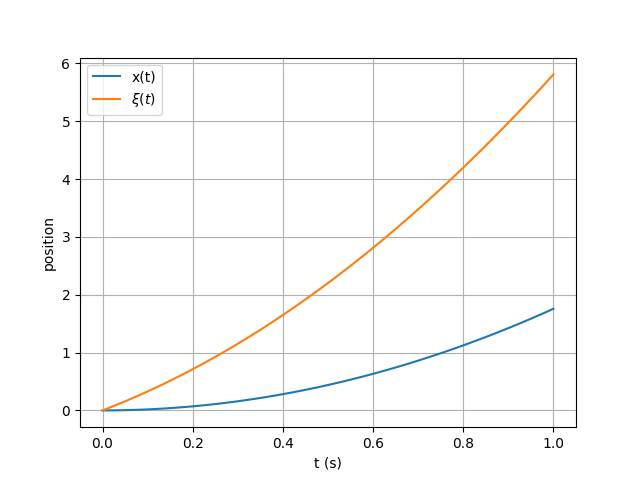
\includegraphics[width=\linewidth]{xxi.png}
          \end{enumerate}
\end{enumerate}

\subsection*{Answer:}

\begin{answer}
    \begin{align}
            (m_1 + m_2 + 3 m_3) \ddot{x} + \ddot{\xi} m_1 \cos(\alpha) = (P_1 + P_2 + 2 P_3) \sin(\alpha) - b \dot{x} \notag \\
            m_1 \ddot{\xi} + m_1 \ddot{x} \cos(\alpha) = P_1 \cos(\alpha) \notag
    \end{align}
\end{answer}